\documentclass[final,5p,times,twocolumn]{elsarticle}

\usepackage{lineno}
\linenumbers

\begin{document}

\begin{frontmatter}

\title{Development of the CBM RICH readout electronics and DAQ}

\author[a]{J.~Adamczewski-Musch}
\author[c]{P.~Akishin}
\author[b]{K.-H.~Becker}
\author[c,f]{S.~Belogurov}
\author[d]{J.~Bendarouach}
\author[e]{N.~Boldyreva}
\author[d]{C.~Deveaux}
\author[e]{V.~Dobyrn}
\author[d]{M.~D\"urr}
\author[a]{J.~Eschke}
\author[b]{J.~F\"ortsch}
\author[d]{J.~Heep}
\author[d]{C.~H\"ohne}
\author[b]{K.-H.~Kampert}
\author[e,f]{L.~Kochenda}
\author[b,d]{J. Kopfer}
\author[e,f]{P.~Kravtsov}
\author[b]{I.~Kres}
\author[d,h]{S.~Lebedev}
\author[d]{E.~Lebedeva}
\author[e]{E.~Leonova}
\author[a]{S.~Linev}
\author[d]{T.~Mahmoud}
\author[g]{J.~Michel}
\author[e]{N.~Miftakhov}
\author[a]{W.~Niebur}
\author[c]{E.~Ovcharenko\corref{cor1}} \ead{eovchar@jinr.ru}
\author[b]{V.~Patel}
\author[b]{C.~Pauly}
\author[b]{D.~Pfeifer}
\author[b]{S.~Querchfeld}
\author[b]{J.~Rautenberg}
\author[b]{S.~Reinecke}
\author[e]{Y.~Riabov}
\author[e]{E.~Roshchin}
\author[e,f,h]{V.~Samsonov}
\author[c,i]{V.~Schetinin}
\author[e]{O.~Tarasenkova}
\author[a]{M.~Traxler}
\author[a]{C.~Ugur}
\author[e]{E.~Vznuzdaev}
\author[e]{M.~Vznuzdaev}

\address[a]{GSI Helmholtzzentrum f\"ur Schwerionenforschung GmbH, D-64291 Darmstadt, Germany}
\address[b]{Department of Physics, University Wuppertal, D-42097 Wuppertal, Germany}
\address[c]{Laboratory of Information Technologies, Joint Institute for Nuclear Research (JINR-LIT), 141980 Dubna, Russia}
\address[d]{Institute of Physics II and Institute of Applied Physics, Justus Liebig University Giessen, D-35392 Giessen, Germany}
\address[e]{National Research Centre - Kurchatov Institute, B.~P.~Konstantinov Petersburg Nuclear Physics Institute, 188300 Gatchina, Russia}
\address[f]{National Research Nuclear University MEPhI (Moscow Engineering Physics Institute), 115409 Moscow, Russia}
\address[g]{Institut f{\"u}r Kernphysik, Goethe University Frankfurt, D-60438 Frankfurt am Main, Germany}
\address[h]{St.~Petersburg State Polytechnic University (SPbSPU), 195251 St.~Petersburg, Russia}
\address[i]{Bauman Moscow State Technical University, 105005 Moscow, Russia}

\cortext[cor1]{Corresponding author}

\begin{abstract}
A real size prototype of the CBM RICH detector was tested in beam at CERN in November 2014 with new readout electronics. A detailed analysis of the timing characteristics of the readout chain  will be presented in this article. Results of the time precision measurements for several subsets of all channels and the stability of the fine time calibration will be discussed. The obtained sub-nanosecond time precision allows also to investigate the effect on timing when using additional wavelength-shifting films on top of the MAPMT windows.
\end{abstract}

\begin{keyword}
CBM; RICH; readout; DAQ; WLS; time precision.
\end{keyword}

\end{frontmatter}

%%%%%%%%%%%%%%%%%%%%%%%%%%%%%%%%%%%%%%%%%%%%%%%%%%%%%%%%%%%%%%%%%%%%%%%%%%%%%%%%%%%%%%%%%%%%%%%%%%%%%%%%%%%%%%%%
\section{Introduction}

The CBM experiment~\cite{CBM} at the future FAIR facility (Darmstadt, Germany)~\cite{FAIR} will investigate strongly interacting matter at high net-baryon densities but moderate temperatures in heavy-ion collisions. The CBM RICH detector is required for identifying electrons in a momentum range up to 8~GeV/c \cite{CBMRICHPROJECT}. The detector consists of gaseous radiator, spherical mirrors and segmented photosensitive camera made of $\approx$1000~Hamamatsu H12700 multi-anode photomultiplier tubes (MAPMT). The MAPMTs will be read out by self-triggered FPGA-based front end boards (FEB) detecting only time information.

During common CBM beam tests at CERN-PS in Nov 2014 a CBM RICH prototype including a camera of 16~MAPMTs partially covered with p-terphenyl as wavelength shifter (WLS, \cite{WLS}) has been successfully tested. The MAPMTs were read out by 64~PADIWA FEBs and digitized by 64~TDCs located at 16~TRB~v3 boards \cite{TRB}. Further readout has been performed via two parallel chains: using FLES \cite{FLES} Interface Board (FLIB) and standard Ethernet via router to Network Interface Card (NIC). Figure~\ref{fig:BeamSetup} shows the scheme of the CBM RICH prototype during the beam tests.

\begin{figure}[tbh]
	\centering
	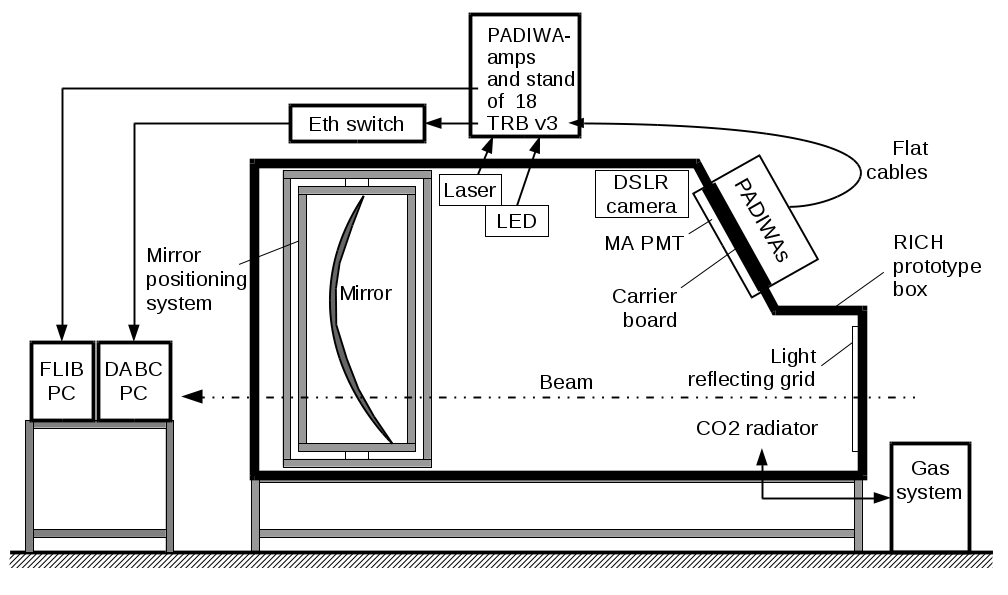
\includegraphics[width=0.48\textwidth]{figures/Beamtime_eng_RICH2016_poster.png}
	\caption{Sketch of the CBM RICH beam test setup.}
	\label{fig:BeamSetup}
\end{figure}

PADIWA is a 16~channel FEB which realizes a preamplifier and a discriminator with an adjustable threshold, the latter inside an FPGA. TRB~v3 is a multifunctional board which employs 5~FPGAs. The main TRB configuration used in CBM RICH has 4~peripheral FPGAs programmed as TDCs \cite{TDC} and 1~central FPGA programmed as HUB. One readout module (see \cite{PEPAN} for more details), consisting of 4~PADIWAs and 1~TRB, is used to read out one 64-pixel MAPMT. Timestamps of the leading and trailing edges of the discriminated signal are detected thus allowing the measurement of time-over-threshold (ToT).

The software for the CBM RICH data processing is implemented in the CbmRoot framework \cite{SEMEN}. All stages from readout to analysis can be performed «on the fly» with or without recording any intermediate information on disk. The data processing pipeline includes the following stages: unpacking, fine time calibration and delay calibration for each channel, hit building, event building, reconstruction and analysis. See refs. \cite{PEPAN} and \cite{RINGS} for more details on the functionality and implementation.

%%%%%%%%%%%%%%%%%%%%%%%%%%%%%%%%%%%%%%%%%%%%%%%%%%%%%%%%%%%%%%%%%%%%%%%%%%%%%%%%%%%%%%%%%%%%%%%%%%%%%%%%%%%%%%%%
\section{Fine time calibration}

The detection of the timestamp in an FPGA-based TDC, used by CBM RICH, is done in two stages. The coarse time is registered using a circular counter which is controlled by the clock with a 5~ns period. The most significant 28~bits are called 'epoch' and the remaining 11~bits are called 'coarse time'. For more precise timestamp measurement an additional 10-bit register is used. The register is filled from the fine time counter implemented using Tapped Delay Line (TDL) on 512~elements.
'Coarse' and 'fine' time are transmitted into DAQ in a single message for each detected edge while the 'epoch' message is only sent once for a group of edges detected in this epoch.
A calibration of the fine time is required to achieve best time precision of 21~ps (see~\cite{FINECALIB,PEPAN}). For each channel, using a subset of the recorded data, a discrete calibration function $ f_{calib}(Fine) $ is built to translate the fine time counter value into the fine time ranging from 0~ns to 5~ns. The full time $ T $ in ns is then computed using the following formula:

{\centering
$ T = Epoch \cdot 2048 \cdot 5ns + Coarse \cdot 5ns - f_{calib}(Fine) $ \\
}

Exact range of possible fine time counter values and non-linearity of the calibration function depend on the technological fluctuations of the FPGA elements. As an example, the difference between the calibration function and its piecewice linear fit is presented in figure~\ref{fig:CalibTableMinusLinear}. The non-linearity does not exceed 60~ps. Figure~\ref{fig:CalibStability} illustrates the stability of this calibration in time. Deflection of calibration functions obtained at three different 2-minute long subsets of data from one, obtained at the complete 15-minute long data set, are shown. Similar stability is observed for longer periods. Typical fluctuations are around 10~ps.

\begin{figure}[tbh]
	\centering
	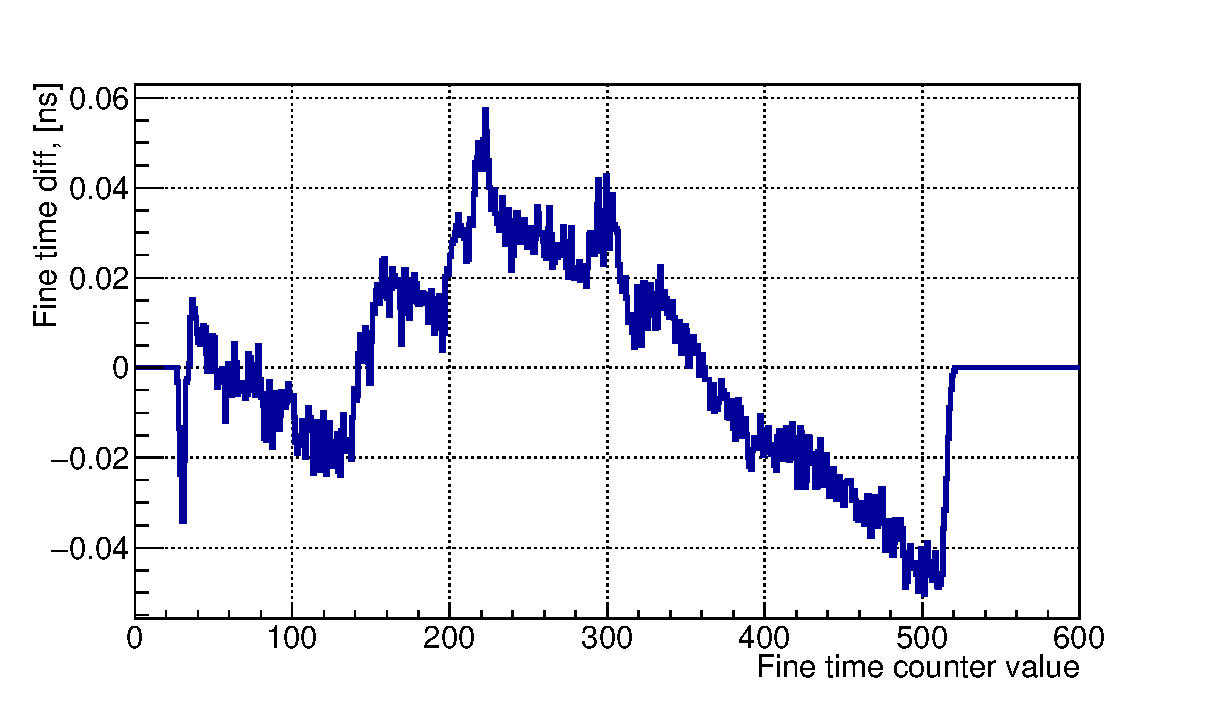
\includegraphics[width=0.48\textwidth]{figures/CalTableMinusFit_0010_01_feb2017.eps}
	\caption{Difference between the measured $ f_{calib} $ and its piecewice linear fit.}
	\label{fig:CalibTableMinusLinear}
\end{figure}

\begin{figure}[tbh]
	\centering
	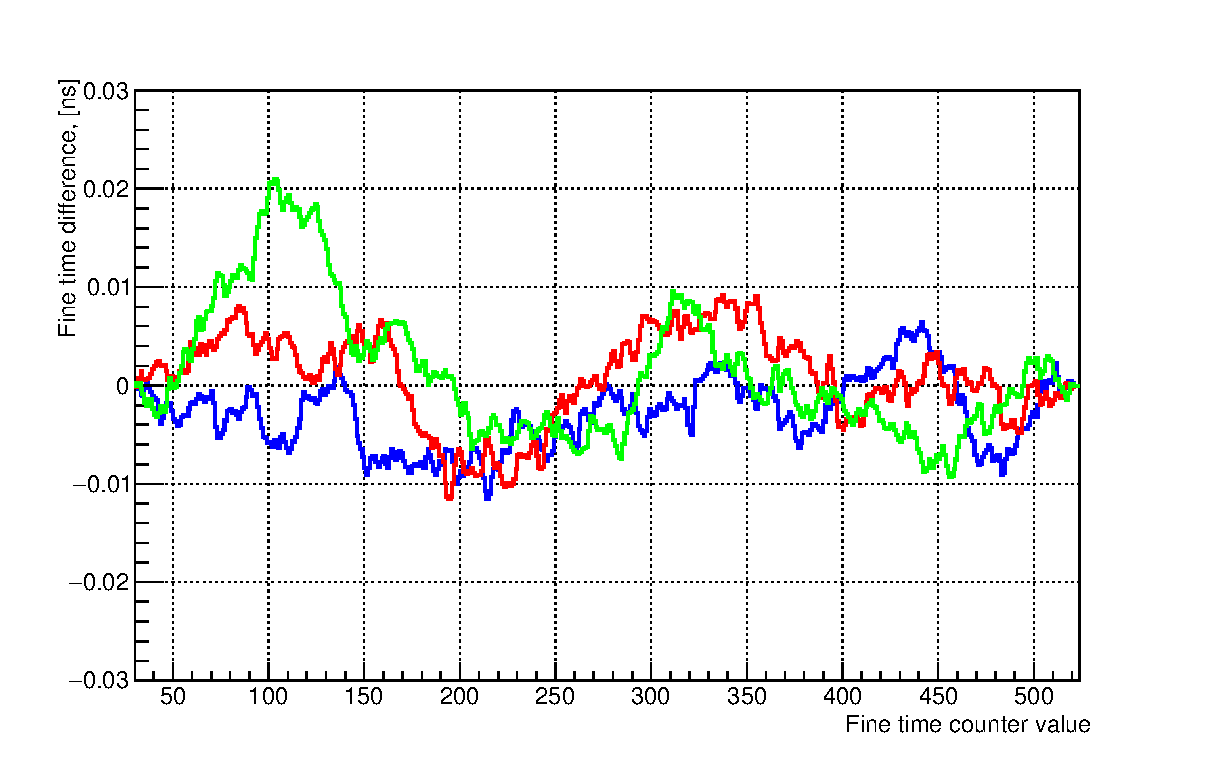
\includegraphics[width=0.48\textwidth]{figures/Stability_01_diff.eps}
	\caption{Deflection of calibration functions obtained at three different subsets of data from one, obtained at the complete data set.}
	\label{fig:CalibStability}
\end{figure}

%%%%%%%%%%%%%%%%%%%%%%%%%%%%%%%%%%%%%%%%%%%%%%%%%%%%%%%%%%%%%%%%%%%%%%%%%%%%%%%%%%%%%%%%%%%%%%%%%%%%%%%%%%%%%%%%
\section{Full readout chain time precision}

The acquired data have been used to determine the time precision of the readout chain. A laser Alphalas Picopower LD405 coupled with the pulser Alphalas PLDD-250 \cite{LASER} was used as a source for fast ($<40$~ps) light flashes. Fine time calibration and channel delay corrections relative to a reference channel were applied to the data. The signals in different channels in one event coming from a laser flash are considered simultaneous.

Figure~\ref{fig:TimePrec} shows the leading edge time difference distributions within one event for four different cases:
between two typical channels (blue), for all possible pairs combined from 16 channels read out by one PADIWA FEB (red), for all possible pairs combined from 64 channel of one MAPMT (green), and  for all possible pairs combined from the top-right quarter of the camera consisting of 4MAPMTs (black).
The distributions have been scaled to make the visual comparison easier. The FWHM and RMS values are listed in table~\ref{tabl:TimePrecTable}.
One can notice less than 100~ps displacements of maxima from zero. Such displacements indicate non-ideal additivity of the channel delay corrections.

Increasing the number of channels under analysis, the FWHM is increasing. The shape of the distribution is approaching a Gaussian distribution. It means that peculiarities of distributions for individual channels are washed out according to the central limit theorem. The reported FWHM values can be considered as $ \sqrt 2 $ times bigger than classically defined time precision because both terms of the time difference are fluctuating independently following similar distributions. Thus our estimation for the time precision is about 1.1~ns for the biggest analyzed subset of channels. This number exceeds the MAPMT transition time jitter (0.28~ns) and is dominated by the walk of the leading edge of the logical signal due to fluctuations of the single photoelectron amplitude. The walk corrections can be introduced if ToT is correctly measured. Unfortunately this was not possible in the current setup, see \cite{PEPAN} for details.

\begin{figure}[tbh]
	\centering
	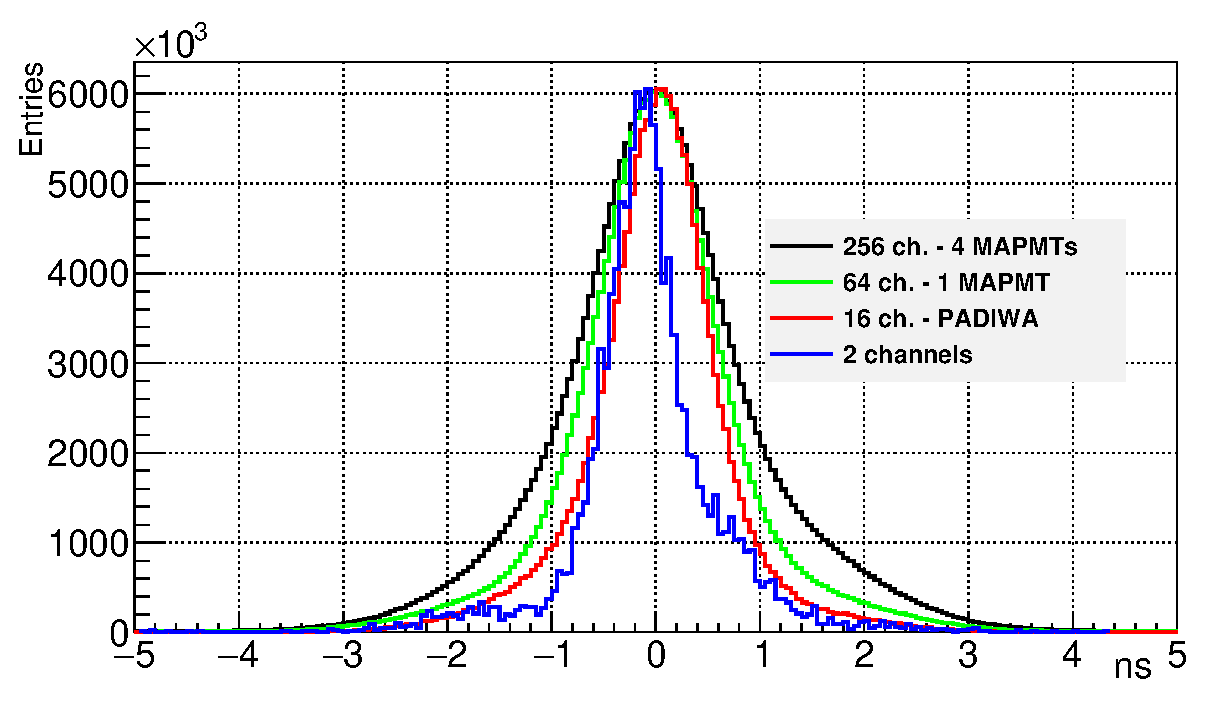
\includegraphics[width=0.45\textwidth]{figures/TimePrecision_evolution_laser_WLSoff_color.eps}
	\caption{The leading edge time difference distributions for different camera areas.}
	\label{fig:TimePrec}
\end{figure}

\begin{table}[tbh]
\centering
	\begin{tabular}{ | p{0.22\linewidth} | p{0.10\linewidth} | p{0.10\linewidth} | p{0.12\linewidth} | p{0.12\linewidth} | }
		\hline		
		\scriptsize{Analyzed area} & \scriptsize{A pair of channels} & \scriptsize{One PADIWA} & \scriptsize{One MAPMT} & \scriptsize{Camera quarter} \\
		\hline
		\scriptsize{Num. of channels} & 2 & 16 & 64 & 256\\
		\hline
		\scriptsize{FWHM, ns} & 0.65 & 1.00 & 1.30 & 1.55\\
		\hline
		\scriptsize{RMS, ns} & 0.699 & 0.713 & 0.894 & 1.034\\
		\hline
	\end{tabular}

	\caption{FWHM and RMS of the leading edge time difference distributions for different analyzed areas.}
	\label{tabl:TimePrecTable}

\end{table}

%%%%%%%%%%%%%%%%%%%%%%%%%%%%%%%%%%%%%%%%%%%%%%%%%%%%%%%%%%%%%%%%%%%%%%%%%%%%%%%%%%%%%%%%%%%%%%%%%%%%%%%%%%%%%%%%
\section{p-terphenyl WLS effect on timing}

Some of MAPMTs in the camera were covered with WLS layers for the first runs, then cleaned and used without WLS films for the second set of runs. Comparing the data received using these MAPMTs before and after cleaning we can analyse the effect of the WLS layer.

A Cherenkov ring reconstructed in a beam event contains in average 16.2~hits without WLS and 19.3~hits with WLS. All the Cherenkov photons in an event can be considered simultaneous. For each Cherenkov ring, the first in time hit is used to define the reference time $ t_{ref} $. For all the other hits in the ring, the relative hit time, $ t'_i = t_i - t_{ref} $, $ i \neq ref $ is computed and histogrammed for all Cherenkov rings in the run. Results for runs with and without WLS are shown in figure~\ref{fig:WLS} as the upper and lower curves correspondingly. Left rising part of both the curves is due to the MAPMT transition time jitter. Fitting the relative hit time distribution without WLS layer with an exponent starting at 0.4~ns, one gets a decay constant of $ \tau_0 = 540$~ps. The upper curve in figure~\ref{fig:WLS} (gray) contains both hits from the Cherenkov photons and the photons emitted by the WLS. The separate time resolved fluorescence measurements with excitation at $\lambda=280$~nm gave for the same WLS film the following time constants: $ \tau_1 = 1.4$~ns, $ \tau_2 = 3.8$~ns, $ \tau_3 = 45$~ns.

The quality of the upper curve in figure~\ref{fig:WLS} does not allow to reliably extract all three WLS time constants from our data, however fixing $ \tau_0$, $\tau_2$ and $\tau_3$ reported above, we get from the fit (red solid line in figure~\ref{fig:WLS}) $\tau_1=1.1$~ns. The difference betwen two results for $\tau_1$ may be attributed either to the systematic uncertainty of the method or to the different spectra of the excitation light.

The fast ($\tau_0$) component comprises about 80\% of all WLS hits. Within a coincidence window of 20~ns 98\% of all hits can be collected when applying WLS layers. Taking into account the foreseen interaction rates, such timing windows are well feasible for the CBM RICH and thus allow to use WLS layers for increasing UV sensitivity of the photodetector.

\begin{figure}[tbh]
	\centering
	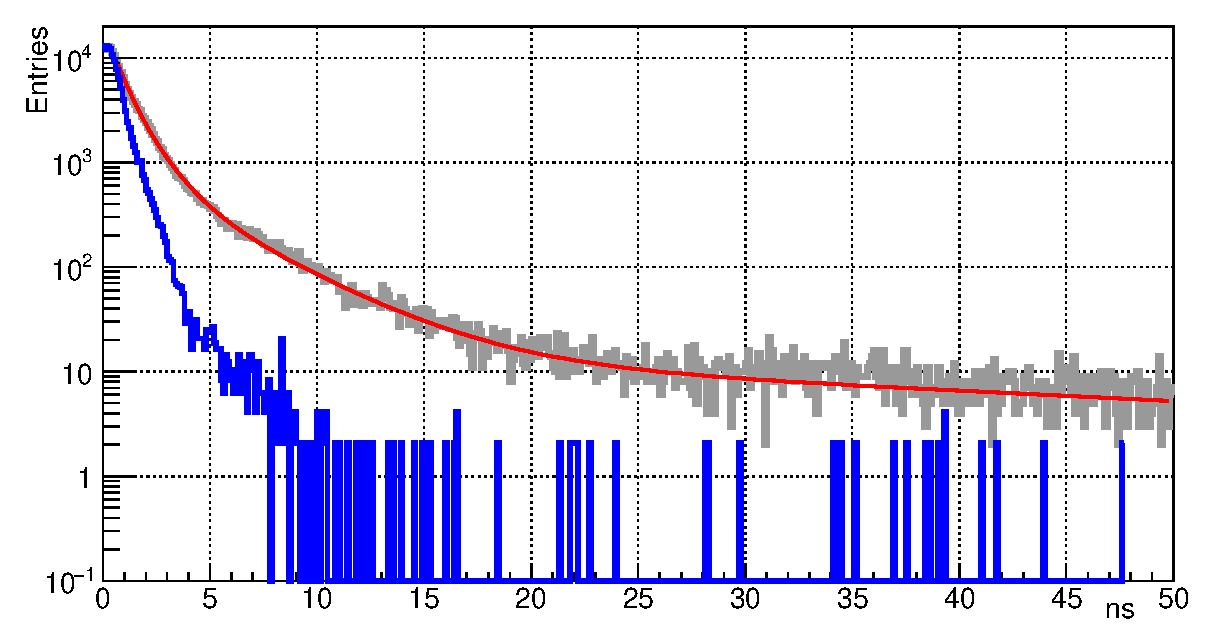
\includegraphics[width=0.48\textwidth]{figures/WLS_on_fitting_with_WLS_off_scaled.eps}
	\caption{Normalized in the maximum relative time distributions of the hits belonging to the Cherenkov rings w.r.t the first in time hit in the ring. Statistic is accumulated over 56000~rings without (blue, lower curve) and 90000 rings with (gray, upper curve) WLS layer. The four-exponential fit to the upper curve is shown as red solid line.}
	\label{fig:WLS}
\end{figure}

%%%%%%%%%%%%%%%%%%%%%%%%%%%%%%%%%%%%%%%%%%%%%%%%%%%%%%%%%%%%%%%%%%%%%%%%%%%%%%%%%%%%%%%%%%%%%%%%%%%%%%%%%%%%%%%%
\section{Summary}

The timing performance of the readout system prototype of the CBM RICH detector has been investigated. The following issues are discussed: accuracy and stability of the TDC calibration; overall time precision within one readout board, one MAPMT and for several MAPMTs; effects due to the wave-length shifting films. The detailed analysis of the readout electronics as presented here led to improvements implemented in the next iteration of the RICH readout which is presented in \cite{PAULY}.

%%%%%%%%%%%%%%%%%%%%%%%%%%%%%%%%%%%%%%%%%%%%%%%%%%%%%%%%%%%%%%%%%%%%%%%%%%%%%%%%%%%%%%%%%%%%%%%%%%%%%%%%%%%%%%%%
\section*{Acknowledgements}

This work was supported by the Hessian LOEWE initiative through the Helmholtz International Center for FAIR (HIC for FAIR), by the Helmholtz Graduate School for Hadron and Ion Research, by the GSI F\&E-Cooperation with Giessen and Wuppertal (WKAMPE1012), by BMBF Grants 05P12RGFCG, 05P12PXFCE, 05P09PXFC5, 05P15PXFCA and 05P15RGFCA, and by the Ministry of Education and Science of the Russian Federation (grant no. 14.A12.31.0002) in accordance with the Russian Federation Government Regulation no. 220.

%%%%%%%%%%%%%%%%%%%%%%%%%%%%%%%%%%%%%%%%%%%%%%%%%%%%%%%%%%%%%%%%%%%%%%%%%%%%%%%%%%%%%%%%%%%%%%%%%%%%%%%%%%%%%%%%
\section*{References}

\begin{thebibliography}{99}

\bibitem{CBM}
C.~Hoehne for the CBM collaboration,
PoS (DIS2016) 272

\bibitem{FAIR}
http://fair-center.eu/

%\bibitem{CBMRICH1}
%C.~Hoehne, et. al.,
%Development of a RICH detector for electron identification in CBM,
%NIM A 595 (2008) 187

%\bibitem{CBMRICH2}
%C.~Hoehne, et. al.,
%Development of a RICH detector for CBM: simulations and experimental tests,
%NIM A 639 (2011) 294

\bibitem{CBMRICHPROJECT}
J. Adamczewski-Musch, et al.,
%The CBM RICH project,
NIM A 766 (2014) 101

\bibitem{WLS}
J. Adamczewski-Musch, et. al.,
%Influence of wavelength-shifting films on multianode PMTs with UV-extended windows,
NIM A 783 (2015) 43

\bibitem{TRB}
A Neiser et al 2013 JINST 8 C12043
%A. Neiser, et. al.,
%TRB3: a 264 channel high precision TDC platform and its applications,
%2013 JINST 8 C12043

\bibitem{FLES}
J de Cuveland et al., 2011 J. Phys.: Conf. Ser. 331 022006
%A First-level Event Selector for the CBM Experiment at FAIR,
%J. de Cuveland, V. Lindenstruth (for the CBM Collaboration)
%2011 J. Phys.: Conf. Ser. 331 022006

\bibitem{TDC}
C. Ugur, et. al.,
%264 Channel TDC Platform Applying 65 Channel High Precision (7.2 ps RMS) FPGA Based TDCs,
10.1109/NoMeTDC.2013.6658234

\bibitem{PEPAN}
J. Adamczewski-Musch, et. al.,
Tests of the CBM RICH readout and DAQ prototype,
submitted to 'PEPAN leters'

\bibitem{SEMEN}
S.~Lebedev et al.,
this issue

\bibitem{RINGS}
S Lebedev et al 2010 J. Phys.: Conf. Ser. 219 032015 
%S. Lebedev, C. Hohne, G. Ososkov,
%Ring Recognition and Electron Identication in the RICH detector of the CBM Experiment at FAIR,
%2010 J. Phys.: Conf. Ser. Vol. 219 032015,
%10.1088/1742-6596/219/3/032015

\bibitem{FINECALIB}
R.~Szplet, J.~Kalisz, and R.~Pelka,
IEEE Trans. Instr. and Meas. 1997(46)449

\bibitem{LASER}
%Laser and pulser official site,
http://www.alphalas.com/products/lasers/ picosecond-pulse-diode-lasers-with-driver-picopower-ld-series.html

\bibitem{PAULY}
C.~Pauly et al.,
this issue

\end{thebibliography}

%%%%%%%%%%%%%%%%%%%%%%%%%%%%%%%%%%%%%%%%%%%%%%%%%%%%%%%%%%%%%%%%%%%%%%%%%%%%%%%%%%%%%%%%%%%%%%%%%%%%%%%%%%%%%%%%

\end{document}